\section{Linear model}

We have seen that the broadcast and reduce operations have different behaviours depending on the number of processes and the message size. In order to explain better the results, we will introduce a model that can help us in getting a better understanding of the performance of these operations.

Let's consider the broadcast operation with linear algorithm and mapping of the processes by core. 

The baseline model determined by the collected data is the following.

\begin{equation}
    Latency = \beta_0 Processes + \beta_1 Size
\end{equation}

\begin{table}[htbp]
    \centering
    \caption{OLS Regression Results}
    \begin{tabular}{lcccccc}
    \hline
    \hline
     & \multicolumn{6}{c}{Dep. Variable: Latency} \\
    \hline
     & Coef. & Std. Err. & t & P \textgreater{} abs(t) & [0.025 & 0.975] \\
    \hline
    Processes & 1.1264 & 0.235 & 4.798 & 0.000 & 0.665 & 1.588 \\
    Size & 0.0011 & 0.000025 & 45.400 & 0.000 & 0.001 & 0.001 \\
    \hline
    \end{tabular}
\end{table}
We do not include a intercept in the model since a message of $0$ byte does not make sense. The $R^2$ achieved by the baseline model is $0.84$ and the AIC is $6096$.
    

By applying some transformations to the data, we can improve the model.
Let's consider the following improved model.

\begin{equation}
    \log_{2}Latency = \beta_0 Processes + \beta_1 \log_{2} Size
\end{equation}

\begin{table}[htbp]
    \centering
    \caption{OLS Regression Results}
    \begin{tabular}{lcccccc}
    \hline
     & \multicolumn{6}{c}{Dep. Variable: log2\_Latency} \\
    \hline
     & Coef. & Std. Err. & t & P \textgreater{} abs(t) & [0.025 & 0.975] \\
    \hline
    Processes & 0.0274 & 0.0040 & 6.693 & 0.000 & 0.019 & 0.035 \\
    log2\_Size & 0.3256 & 0.0098 & 33.346 & 0.000 & 0.306 & 0.345 \\
    \hline
    \end{tabular}
\end{table}

The improved model, is characterized by a $R^2$ of $0.88$ and the AIC is $1842$. The second model is able to explain the data better than the baseline model. The $R^2$ is higher and the AIC is lower.

This model allow us to understand the behaviour of the broadcast operation with linear algorithm and mapping of the processes by core. The interesting results are the following:
\begin{itemize}
    \item an increase of one unit in the number of the processes, leads to and increase of $2^{0.0274} \approx 1.01$ in the latency;
    \item an increase of one unit in the message size, leads to an increase of $0.3256$ in the latency.
\end{itemize}

\begin{figure}[h!]
    \centering
    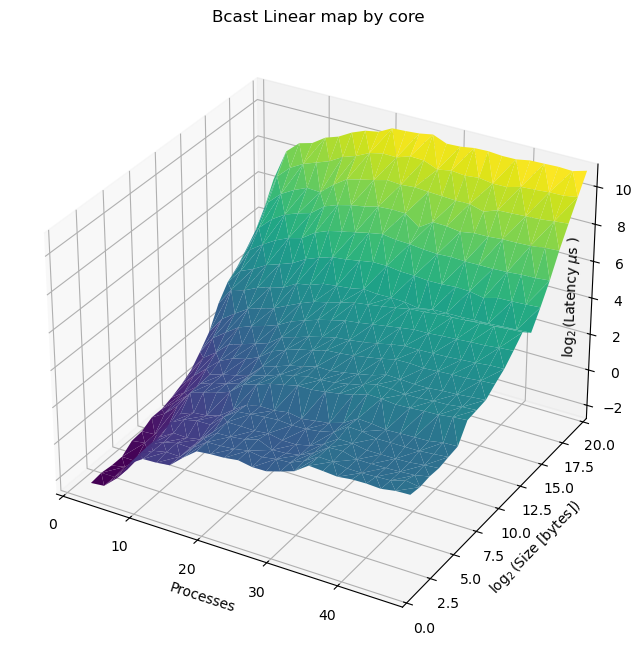
\includegraphics[width=0.8\textwidth]{../plots/bcast_linear_core_3d.png}
    \caption{3D plot of the broadcast operation with linear algorithm and mapping of the processes by core. The plot shows the relationship between the number of processes, the logartihm of message size and the logarithm of the latency.}
\end{figure}